\documentclass[11pt,german,hideothersubsections]{beamer}

\usepackage{hyperref}
\usepackage{amsmath,nicefrac,booktabs,mathabx}
\usepackage{natbib}
\usepackage{url}
\usepackage{textpos}
\usepackage{listings}
\definecolor{Rblau}{rgb}{.3,.6,.9}

\lstset{language=R,
        basicstyle=\ttfamily\footnotesize,
        keywordstyle=\color{blue}\bfseries,
        identifierstyle=\color{Rblau},
        commentstyle=\color{gray},
        stringstyle=\color{green}\ttfamily,
        showstringspaces=false,
        frame=tb}



\bibpunct{(}{)}{;}{a}{,}{,}
\usepackage[english]{babel}
\usepackage[latin1]{inputenc}
\usepackage{helvet}
\usepackage{graphicx}
\usepackage{color}
\usepackage{multirow,dcolumn}
\usepackage{ragged2e}
\usepackage{xcolor}
\usepackage{colortbl}
\usepackage{tikz}
\usetikzlibrary{calc}
\usepackage{booktabs}
\colorlet{tablesubheadcolor}{gray!25}
\colorlet{tableheadcolor}{gray!40}
\colorlet{tablerowcolor}{gray!15.0}
\usetheme[english]{Gesis}
\setbeamertemplate{navigation symbols}{}
\setbeamertemplate{footline}[frame number]%{\hspace*{.2cm}\insertframenumber}
\setbeamerfont{caption}{size=\footnotesize}
\usefonttheme[onlylarge]{structuresmallcapsserif} % alte Schrift

\newcommand{\R}[1]{{\tt \color{blue}  #1}}
\newtheorem{thm}{Theorem}
\newtheorem{rem}{Bemerkung}
\newtheorem{lem}{Lemma}

\definecolor{hellgrau}{rgb}   {0.109375,  0.40625,   0.51953125}
\definecolor{dunkelgrau}{rgb} {0.009375,  0.30625,   0.41953125}
\definecolor{dunkelgrau2}{rgb}{0.009375,  0.20625,   0.31953125}
\definecolor{hellbraun}{rgb}  {0.9140625, 0.8984375, 0.8046875}
\definecolor{hellbraun2}{rgb} {.95,       0.9,       0.8}
\definecolor{alertred}{rgb}   {0.8515625, 0.3828125, 0.08984375}
\definecolor{orange}{rgb}{1,0.5,0}


\setbeamercolor{firstsecslide}{fg=white,bg=dunkelgrau}
\setbeamertemplate{blocks}[rounded][shadow=true]

\newcolumntype{d}[0]{D{,}{.}{6}}

\newenvironment{itemizeol}{\begin{itemize}[<+->]}{\end{itemize}}
\newenvironment{descriptionol}{\begin{description}[<+->]}{\end{description}}

\newcolumntype{V}[1]{%
  >{\RaggedRight\hspace{0pt}}p{#1}%
}

\newcommand{\emphred}[1]{\textcolor{alertred}{#1}}
\newcommand{\emphcol}[1]{\textcolor{dunkelgrau}{\slshape #1}}

\setcounter{tocdepth}{1}
\setbeamercolor*{section in toc}{fg=hellgrau}
\setbeamertemplate{bibliography item}[default]
\makeatother
\addtobeamertemplate{frametitle}{}{%
\begin{textblock*}{100mm}(.91\textwidth,-1cm)

\includegraphics[height=1cm,width=2cm]{../../graphs/logos/GESIS_Logo_kompakt_en.jpg}
\end{textblock*}}

\title[Day 1]{Tutorial: Sampling, Weighting and Estimation\\ \Large{Day 4} }
%\subtitle{Umgang am Beispiel von Telefonstichproben}

\author[M. Sand]{Stefan Zins, Matthias Sand\\ and Jan-Philipp Kolb\\ \vspace{.5cm} \footnotesize{GESIS - Leibniz Institute\\ for the Social Sciences}}
%\institute{\includegraphics[width=4.5cm]{GESIS_Logo_informell}}
\date[]{\color{dunkelgrau}\footnotesize%
\begin{minipage}{8cm}%
\begin{center}%
\scriptsize{
\textbf{GESIS Summer School}\\ \tiny{Cologne, Germany}%
}\\
\vspace{0.25cm}
\textbf{August 27th, 2015}%

\end{center}%
\end{minipage}}%


\usepackage{Sweave}
\begin{document}
\Sconcordance{concordance:Day4.tex:Day4.Rnw:%
1 99 1 1 0 2 1 1 15 7 1 1 21 2 1 1 2 1 0 1 1 7 0 1 1 7 0 1 2 2 1 1 2 8 %
0 1 2 13 1 1 2 25 0 1 2 11 1 1 2 4 0 1 2 15 1 1 2 1 0 1 1 10 0 1 2 3 1 %
1 3 5 0 1 2 15 1 1 3 1 2 10 1 1 2 1 0 1 1 9 0 1 2 36 1 1 2 1 0 1 1 7 0 %
2 1 9 0 1 2 15 1 1 2 1 0 1 1 1 2 7 0 1 2 14 1 1 2 1 0 1 1 1 2 1 0 1 1 %
12 0 1 2 17 1 1 3 8 0 1 2 13 1 1 3 12 0 1 4 4 0 1 2 26 1 1 3 2 0 1 1 1 %
2 16 0 1 2 16 1 1 3 2 0 1 2 16 0 1 2 18 1 1 3 2 0 1 1 1 2 16 0 1 2 32 1 %
1 2 25 0 1 2 10 1 1 2 1 0 1 1 23 0 1 2 97 1}

\maketitle
%%%%%%%%%%%%%%%%%%%%%%%%%%%%%%%%%%%%%%%%%%%%%%%%%%%%%%%%
\begin{frame}[fragile]{Usefull Commands} {of the Survey Package}
%\frametitle{\vspace{-.05cm}\begin{center}\footnotesize{Usefull Commands of the Survey Package}\end{center}}
\footnotesize{
\vspace{-.25cm}
\begin{center}
\textbf{Computation of contrasts}
\end{center}
\begin{itemize}
\item Using the multi-stage sample of day 3 (\R{mul.surv})
\end{itemize}
\begin{Schunk}
\begin{Sinput}
 means <-svymean(~api00+api99,mul.surv)
 means
\end{Sinput}
\begin{Soutput}
      mean   SE
api00  644 11.4
api99  613 13.2
\end{Soutput}
\begin{Sinput}
 svycontrast(means,quote(api00-api99))
\end{Sinput}
\begin{Soutput}
         nlcon   SE
contrast  30.6 3.19
\end{Soutput}
\end{Schunk}
\begin{itemize}
\item The command \R{svycontrast()} can be used to estimate contrasts for linear and nonlinear survey statistics and their standard error
\end{itemize}
\begin{Schunk}
\begin{Sinput}
 svycontrast(means,quote(api00/api99))
\end{Sinput}
\begin{Soutput}
         nlcon   SE
contrast  1.05 0.01
\end{Soutput}
\end{Schunk}
\begin{itemize}
\item[$\Rightarrow$] \R{svyratio(\textasciitilde0 api00,\textasciitilde0 api99,mul.surv)} generates the same results
\end{itemize}
}
\end{frame}

%%%%%%%%%%%%%%%%%%%%%%%%%%%%%%%%%%%%%%%%%%%%%%%%%%%%%%%%
\begin{frame}[fragile]{Usefull Commands} {of the Survey Package}
%\frametitle{\vspace{-.05cm}\begin{center}\footnotesize{Usefull Commands of the Survey Package}\end{center}}
\footnotesize{
\begin{center}
\textbf{Weighted regression}
\end{center}
\scriptsize{
\begin{Schunk}
\begin{Sinput}
 summary(svyglm(api00~enroll+meals+api99,mul.surv))
\end{Sinput}
\begin{Soutput}
Call:
svyglm(formula = api00 ~ enroll + meals + api99, mul.surv)

Survey design:
svydesign(id = ~cds + id, fpc = ~fpc + fpc2, strata = NULL, data = DATA.s, 
    pps = "brewer")

Coefficients:
             Estimate Std. Error t value Pr(>|t|)    
(Intercept) 114.31730   38.64877    2.96   0.0049 ** 
enroll       -0.00535    0.00472   -1.13   0.2623    
meals         0.06558    0.18715    0.35   0.7277    
api99         0.86531    0.04505   19.21   <2e-16 ***
---
Signif. codes:  0 '***' 0.001 '**' 0.01 '*' 0.05 '.' 0.1 ' ' 1

(Dispersion parameter for gaussian family taken to be 406.9)

Number of Fisher Scoring iterations: 2
\end{Soutput}
\end{Schunk}
}
}
\end{frame}

%%%%%%%%%%%%%%%%%%%%%%%%%%%%%%%%%%%%%%%%%%%%%%%%%%%%%%%%
\begin{frame}[fragile]{Usefull Commands} {of the Survey Package}
%\frametitle{\vspace{-.05cm}\begin{center}\footnotesize{Usefull Commands of the Survey Package}\end{center}}
\footnotesize{
\begin{center}
\textbf{Weighted regression}
\end{center}

\begin{Schunk}
\begin{Sinput}
 summary(svyglm(api00~enroll+meals+api99,mul.surv))
\end{Sinput}
\end{Schunk}

\begin{itemize}\footnotesize{
\item The \R{svyglm()} function fits linear and generalized lin. models to the data stored in a survey object 
\item syntax almost identical to the glm, except that the data argument is replaced by a design argument $\rightarrow$ weighted least square
\item Main difference to \R{glm()}: \R{svyglm()} doe not use a maximum likelihood approach}
\end{itemize}
}
\end{frame}

%%%%%%%%%%%%%%%%%%%%%%%%%%%%%%%%%%%%%%%%%%%%%%%%%%%%%%%%
\begin{frame}[fragile]{Usefull Commands} {of the Survey Package}
%\frametitle{\vspace{-.05cm}\begin{center}\footnotesize{Usefull Commands of the Survey Package}\end{center}}
\footnotesize{
\begin{center}
\textbf{Survey weighted contingency tables and chi squared tests}
\end{center}
\begin{Schunk}
\begin{Sinput}
 tab1 <- svytable(~stype+sch.wide,mul.surv)
 tab1
\end{Sinput}
\begin{Soutput}
     sch.wide
stype    No   Yes
    E  2003 62108
    H  2003 10441
    M  8014 16028
\end{Soutput}
\end{Schunk}
\begin{itemize}\footnotesize{
\item Creates the weighted contingency table of two or more variables}
\end{itemize}\footnotesize{

\begin{Schunk}
\begin{Sinput}
 plot(tab1, col="blue",xlab = "school type", 
+      ylab = "growth target",cex.lab=0.25)
\end{Sinput}
\end{Schunk}
}
\begin{itemize}
\item Such contingency tables can easily be visualized to learn more about the sampled variables
\end{itemize}

}
\end{frame}

%%%%%%%%%%%%%%%%%%%%%%%%%%%%%%%%%%%%%%%%%%%%%%%%%%%%%%%%
\begin{frame}[fragile]{Usefull Commands} {of the Survey Package}
%\frametitle{\vspace{-.05cm}\begin{center}\footnotesize{Usefull Commands of the Survey Package}\end{center}}
\footnotesize{
\begin{center}
\textbf{Survey weighted contingency tables and chi squared tests}
\end{center}

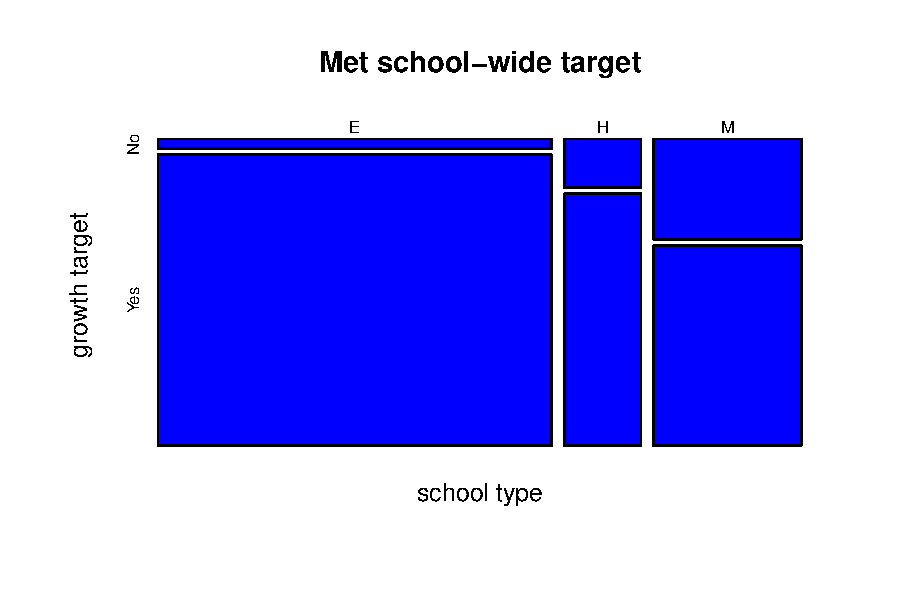
\includegraphics{Day4-009}

}
\end{frame}
%%%%%%%%%%%%%%%%%%%%%%%%%%%%%%%%%%%%%%%%%%%%%%%%%%%%%%%%
\begin{frame}[fragile]{Usefull Commands} {of the Survey Package}
%\frametitle{\vspace{-.05cm}\begin{center}\footnotesize{Usefull Commands of the Survey Package}\end{center}}
\footnotesize{
\begin{center}
\textbf{Survey weighted contingency tables and chi squared tests}
\end{center}
\vspace{.25cm}
\begin{Schunk}
\begin{Sinput}
 chi <- svychisq(~stype+sch.wide,mul.surv,statistic="adjWald")
 chi
\end{Sinput}
\begin{Soutput}
	Design-based Wald test of association

data:  svychisq(~stype + sch.wide, mul.surv, statistic = "adjWald")
F = 4.071, ndf = 2, ddf = 48, p-value = 0.02327
\end{Soutput}
\end{Schunk}
}

\begin{itemize}\footnotesize{
\item Tests for the association of sample variables
\item Numerous tests are applicable
\item In this case it is tested for independence under the consideration of the number of PSUs}
\end{itemize}
\end{frame}
%%%%%%%%%%%%%%%%%%%%%%%%%%%%%%%%%%%%%%%%%%%%%%%%%%%%%%%%
\begin{frame}[fragile]{Usefull Commands} {of the Survey Package}
\footnotesize{
\begin{center}
\textbf{Estimation of subpopulations}
\end{center}
\begin{itemize}
\footnotesize{
\item Within a stratified random sample, subtotals for each stratum are easy to compute, since every stratum can be treated like a separate srs
\pause\item For an unstratified design or subpopulations that are no strata, the situation is more complicated, since the joint inclusion probabilities $\pi_{kl}$ are unequal to those that would be, if this group had been a stratum
\item Sampling weights would be correct, but pairwise sampling probability would be incorrect
\pause\item[$\Rightarrow$] Unbiased point estimates; but standard errors would be wrong
}
\end{itemize}

}
\end{frame}
%%%%%%%%%%%%%%%%%%%%%%%%%%%%%%%%%%%%%%%%%%%%%%%%%%%%%%%%
\begin{frame}[fragile]{Usefull Commands} {of the Survey Package}
\footnotesize{
\begin{center}
\textbf{Estimation of subpopulations}
\end{center}
\begin{itemize}
\footnotesize{
\item The survey package deals with these problems without any further specification as long as the full sample is used to define a survey object
\item Subpopulations either by \R{subset} or \R{svyby}
}
\end{itemize}
\begin{Schunk}
\begin{Sinput}
 sub1 <- subset(mul.surv,sch.wide=="Yes")
 svymean(~api00+api99,sub1)
\end{Sinput}
\begin{Soutput}
      mean   SE
api00  638 12.7
api99  602 14.4
\end{Soutput}
\begin{Sinput}
 sub2 <- svyby(~api00,~stype,svymean,design = mul.surv)
 print(sub2)
\end{Sinput}
\begin{Soutput}
  stype api00    se
E     E 645.1 16.69
H     H 619.9 11.10
M     M 653.6 16.26
\end{Soutput}
\end{Schunk}

}
\end{frame}
%%%%%%%%%%%%%%%%%%%%%%%%%%%%%%%%%%%%%%%%%%%%%%%%%%%%%%%%
\begin{frame}[fragile]{Taylor Linearization} {with the ratio estimator}
%\frametitle{\vspace{-.05cm}\begin{center}\footnotesize{Usefull Commands of the Survey Package}\end{center}}
\footnotesize{
\begin{center}
\textbf{The ratio estimator}
\end{center}
\begin{equation*}
\frac{\hat{t}_{y,HT}}{\hat{t}_{x,HT}}
\end{equation*}
\begin{itemize}
\item Drawing a sample of $n=130$ from bm
\end{itemize}
\begin{Schunk}
\begin{Sinput}
 bm$pik <- inclusionprobabilities(bm$Tot03,130)
 s <- UPmaxentropy(bm$pik)
 ratioest(y=bm$TaxableIncome[s==1],x=bm$averageincome[s==1],
+          Tx=sum(bm$averageincome),pik=bm$pik[s==1])
\end{Sinput}
\begin{Soutput}
[1] 1.385e+11
\end{Soutput}
\end{Schunk}

\begin{itemize}
\item Returns the ratio estimator of the population total
\item[$\Rightarrow$] Another way to calculate the ratio estimator is implemented in the survey package
\end{itemize}
}
\end{frame}

%%%%%%%%%%%%%%%%%%%%%%%%%%%%%%%%%%%%%%%%%%%%%%%%%%%%%%%%
\begin{frame}[fragile]{Taylor Linearization} {with the ratio estimator}
%\frametitle{\vspace{-.05cm}\begin{center}\footnotesize{Usefull Commands of the Survey Package}\end{center}}
\footnotesize{
\begin{center}
\textbf{The ratio estimator}
\end{center}
\begin{Schunk}
\begin{Sinput}
 samp <- bm[s==1,]
 IPkl <-UPmaxentropypi2(bm$pik)
 obj <- svydesign(id=~1,fpc = ~pik,data=samp,
+                  pps = ppsmat(IPkl[s==1,s==1]),variance="YG")
 svyratio(~TaxableIncome,~averageincome,obj)
\end{Sinput}
\begin{Soutput}
Ratio estimator: svyratio.pps(~TaxableIncome, ~averageincome, obj)
Ratios=
              averageincome
TaxableIncome          9370
SEs=
              averageincome
TaxableIncome         474.5
\end{Soutput}
\end{Schunk}
\begin{itemize}
\item The \R{svyratio()} command returns the ratio between the two weighted sampling variables.
%\item[$\Rightarrow$] To obtain an estimator for the total, the ratio must be multiplied with the populatiopn total of the auxiliary variable
\end{itemize}
}
\end{frame}
%%%%%%%%%%%%%%%%%%%%%%%%%%%%%%%%%%%%%%%%%%%%%%%%%%%%%%%%
\begin{frame}[fragile]{Taylor Linearization} {with the ratio estimator}
%\frametitle{\vspace{-.05cm}\begin{center}\footnotesize{Usefull Commands of the Survey Package}\end{center}}
\footnotesize{
\begin{center}
\textbf{The ratio estimator}
\end{center}
\begin{itemize}
%\item The \R{svyratio()} command returns the ratio between the two weighted sampling variables.
\item To obtain an estimator for the total, the ratio must be multiplied with the population total of the auxiliary variable
\end{itemize}

\begin{Schunk}
\begin{Sinput}
 as.numeric(svyratio(~TaxableIncome,~averageincome,obj))*
+   sum(bm$averageincome)
\end{Sinput}
\begin{Soutput}
[1] 1.385e+11 3.327e+12
\end{Soutput}
\end{Schunk}

}
\end{frame}
%%%%%%%%%%%%%%%%%%%%%%%%%%%%%%%%%%%%%%%%%%%%%%%%%%%%%%%%
\begin{frame}[fragile]{Taylor Linearization} {with the ratio estimator}
%\frametitle{\vspace{-.05cm}\begin{center}\footnotesize{Usefull Commands of the Survey Package}\end{center}}
\footnotesize{
\begin{center}
\textbf{Variance estimation}
\end{center}
\begin{itemize}
\item Estimating the Variance of the ratio estimator via \emph{Taylor Linearization} with the sampling package
\end{itemize}
\scriptsize{
\begin{Schunk}
\begin{Sinput}
 vartaylor_ratio(Ys=samp$TaxableIncome,Xs=samp$averageincome,
+                 pikls = IPkl[s==1,s==1])
\end{Sinput}
\begin{Soutput}
$ratio
[1] 9370

$estvar
[1] 234061
\end{Soutput}
\end{Schunk}
\begin{Schunk}
\begin{Soutput}
[1] 483.8
\end{Soutput}
\end{Schunk}
}
\begin{itemize}
\pause\item The survey package uses \emph{Taylor Linearization} by default to estimate standard errors based on design information
\pause\item The \R{vartaylor\_ratio()} returns the HT-estimator of the variance, not the YG-type
\end{itemize}
}
\end{frame}
%%%%%%%%%%%%%%%%%%%%%%%%%%%%%%%%%%%%%%%%%%%%%%%%%%%%%%%%
\begin{frame}[fragile]{Replicate Weights}
%\frametitle{\vspace{-.05cm}\begin{center}\footnotesize{Usefull Commands of the Survey Package}\end{center}}
\footnotesize{
\begin{itemize}
\item Within the survey package all of the \emph{common} strategies are implemented and easy to use
\item First step: redefine the survey object as a replicate weights object with the \R{as.svrepdesign()} command
\item Second step: choosing a strategy with the \R{type=} argument
\pause\item[$\Rightarrow$] Most of the strategies cannot create replicate weights under unequal inclusion probabilities and resample only the PSUs to create replicate weights
\end{itemize}
}
\end{frame}
%%%%%%%%%%%%%%%%%%%%%%%%%%%%%%%%%%%%%%%%%%%%%%%%%%%%%%%%

\begin{frame}[fragile]{Replicate Weights}
%\frametitle{\vspace{-.05cm}\begin{center}\footnotesize{Usefull Commands of the Survey Package}\end{center}}
\footnotesize{
\begin{center}
\textbf{Jackknife}
\end{center}
\begin{Schunk}
\begin{Sinput}
 dclus1 <- svydesign(id=~dnum,weights=~pw,data=apiclus1,
+                     fpc= rep(757/15,times=nrow(apiclus1)))
 clus.rep <- as.svrepdesign(dclus1,type = "JK1")
 svyquantile(~api00 , clus.rep, c (.25 ,.5 ,.75) ,
+             interval.type ="probability")
\end{Sinput}
\begin{Soutput}
Statistic:
      api00
q0.25 551.8
q0.5  652.0
q0.75 717.5
SE:
      api00
q0.25 30.34
q0.5  34.21
q0.75 15.83
\end{Soutput}
\end{Schunk}
\begin{itemize}
\item Allows the estimation of standard errors for quantiles, etc.
\item In case of estimates for the totals and means, the estimates for the standard error are comparable to those of the Taylor Linearization
\item \R{"auto"} as \R{type}-argument uses JKn for stratified and JK1 for unstratified samples
\end{itemize}


}
\end{frame}
%%%%%%%%%%%%%%%%%%%%%%%%%%%%%%%%%%%%%%%%%%%%%%%%%%%%%%%%

\begin{frame}[fragile]{Replicate Weights}
%\frametitle{\vspace{-.05cm}\begin{center}\footnotesize{Usefull Commands of the Survey Package}\end{center}}
\footnotesize{
\begin{center}
\textbf{Bootstrap}
\end{center}
\begin{Schunk}
\begin{Sinput}
 rep.clus2 <- as.svrepdesign(dclus1,type = "bootstrap",
+                             replicates = 100)
 svyquantile(~api00,rep.clus2,c (.25 ,.5 ,.75) ,
+             interval.type ="probability")
\end{Sinput}
\begin{Soutput}
Statistic:
      api00
q0.25 551.8
q0.5  652.0
q0.75 717.5
SE:
      api00
q0.25 29.33
q0.5  30.90
q0.75 15.75
\end{Soutput}
\end{Schunk}
\begin{itemize}
\item[$\Rightarrow$] Reduces the standard error
\item design weights are the starting weights multiplied by the times they have been sampled within each iteration (srswr!)
\end{itemize}
}
\end{frame}
%%%%%%%%%%%%%%%%%%%%%%%%%%%%%%%%%%%%%%%%%%%%%%%%%%%%%%%%%%%%%
\begin{frame}[fragile]{Replicate Weights}
%\frametitle{\vspace{-.05cm}\begin{center}\footnotesize{Usefull Commands of the Survey Package}\end{center}}
\footnotesize{
\begin{center}
\textbf{Balanced Repeated Replicates (BRR)}
\end{center}
\begin{itemize}
\item BRR is appealing because it requires less computational effort than the Jackknife method
\item BRR standard errors are valid for quantiles and median, while the Jackknife method might produce invalid results
\end{itemize}

\scriptsize{
\begin{Schunk}
\begin{Sinput}
 dstrat <- svydesign(id=~1,weights=~pw,strata = ~stype,
+                     data = apistrat,fpc = ~fpc) 
 rep3 <- as.svrepdesign(dstrat,type = "BRR")
 svyquantile(~api00,rep3,c (.25 ,.5 ,.75) ,
+              interval.type ="probability")
\end{Sinput}
\begin{Soutput}
Statistic:
      api00
q0.25 562.2
q0.5  667.2
q0.75 755.1
SE:
      api00
q0.25 15.05
q0.5  11.33
q0.75 13.18
\end{Soutput}
\end{Schunk}
}

}
\end{frame}
%%%%%%%%%%%%%%%%%%%%%%%%%%%%%%%%%%%%%%%%%%%%%%%%%%%%%%%%%%%%%
\begin{frame}[fragile]{Replicate Weights}
\footnotesize{
\begin{center}
\textbf{Summary: replicate weights and single stage sampling}
\end{center}
\begin{itemize}
\item All three methods can only be applied to single-stage samples or resample only on the PSU-level
\item All three approaches ignore the fpc
\pause\item Bootstrap is only straightforward, when all strata sizes are large
\pause\item The BRR approach yields the smallest estimates for the standard error, but has difficulties when dealing with cluster samples
\pause\item[$\Rightarrow$] BRR can only be applied for samples with two clusters per stratum
\pause\item[$\Rightarrow$] All three approaches have problems with multi-stage samples and unequal inclusion probabilities 

\end{itemize}
}
\end{frame}

%%%%%%%%%%%%%%%%%%%%%%%%%%%%%%%%%%%%%%%%%%%%%%%%%%%%%%%%%%%%%
\begin{frame}[fragile]{Replicate Weights}
\footnotesize{
\begin{center}
\textbf{Multi-stage samples and replicate weights}
\end{center}
\begin{itemize}
\item In case of multi-stage samples, the \emph{mrb} or \emph{mrbbootstrap} method of Preston should be employed
\item[$\Rightarrow$] Resamples PSUs and SSUs rather than only PSUs
\end{itemize}
\tiny{
\begin{Schunk}
\begin{Sinput}
 summary(svyglm(api00~enroll+meals+api99,mul.surv))
\end{Sinput}
\begin{Soutput}
Call:
svyglm(formula = api00 ~ enroll + meals + api99, mul.surv)

Survey design:
svydesign(id = ~cds + id, fpc = ~fpc + fpc2, strata = NULL, data = DATA.s, 
    pps = "brewer")

Coefficients:
             Estimate Std. Error t value Pr(>|t|)    
(Intercept) 114.31730   38.64877    2.96   0.0049 ** 
enroll       -0.00535    0.00472   -1.13   0.2623    
meals         0.06558    0.18715    0.35   0.7277    
api99         0.86531    0.04505   19.21   <2e-16 ***
---
Signif. codes:  0 '***' 0.001 '**' 0.01 '*' 0.05 '.' 0.1 ' ' 1

(Dispersion parameter for gaussian family taken to be 406.9)

Number of Fisher Scoring iterations: 2
\end{Soutput}
\end{Schunk}
}

}
\end{frame}
%%%%%%%%%%%%%%%%%%%%%%%%%%%%%%%%%%%%%%%%%%%%%%%%%%%%%%%%%%%%%
\begin{frame}[fragile]{Replicate Weights}
\footnotesize{
\begin{center}
\textbf{Multi-stage samples and replicate weights}
\end{center}
\tiny{
\begin{Schunk}
\begin{Sinput}
 rep4 <- as.svrepdesign(mul.surv,type = "mrbbootstrap")
 summary(svyglm(api00~enroll+meals+api99,rep4))
\end{Sinput}
\begin{Soutput}
Call:
svyglm(formula = api00 ~ enroll + meals + api99, rep4)

Survey design:
as.svrepdesign(mul.surv, type = "mrbbootstrap")

Coefficients:
             Estimate Std. Error t value Pr(>|t|)    
(Intercept) 114.31730   19.95635    5.73  7.4e-07 ***
enroll       -0.00535    0.00256   -2.09    0.042 *  
meals         0.06558    0.09243    0.71    0.482    
api99         0.86531    0.02384   36.30  < 2e-16 ***
---
Signif. codes:  0 '***' 0.001 '**' 0.01 '*' 0.05 '.' 0.1 ' ' 1

(Dispersion parameter for gaussian family taken to be 406.7)

Number of Fisher Scoring iterations: 2
\end{Soutput}
\end{Schunk}
}
\begin{itemize}\scriptsize{
\item Reduces standard error of the estimates
\item Estimates are far more significant
\item Needs more computational time then other resampling strategies
\item[$\Rightarrow$] But: correct approach for multi-stage samples}
\end{itemize}
}
\end{frame}



% apiclus1.  <- apiclus1[!(apiclus1$dnum%in%c(716,413)),]
% apiclus1.$fpc  <- length(unique(apipop$dnum))
% apiclus1.$fpc2 <- table(apiclus1.$dnum)[as.character(apiclus1.$dnum)]
% 
% nh<-round(table(apiclus1.$dnum)/nrow(apiclus1.) *40)
% test <- mapply(function(x,y)sample(as.character(x),y),split(apiclus1.$cds,apiclus1.$dnum)[names(nh)],nh)
% apiclus1.2 <- apiclus1.[apiclus1.$cds%in%unlist(test),]
% 
% vs1 <- svydesign(id=~dnum+cds,fpc=~fpc+fpc2, data = apiclus1.2)
% 
% vs2 <-as.svrepdesign(vs1,type="mrb")
% 
% 
%' <<>>=
%' sv2 <- as.svrepdesign2(mul.surv,type="mrbbootstrap")
%' a<-hadamard(2)
%' @
%' 
%' sv2 <- as.svrepdesign2(mul.surv,type="mrbbootstrap")
%' % summary(svyglm(api00~enroll+meals+api99,sv2))
%' 
%' 
%' summary(svyglm(api00~enroll+meals+api99,sv2))






























































\end{document}
